\subsection{Sémantické parsování pomocí gramatik}\label{subsec:moje_gramatiky}
Extrakce sémantické informace byla jednou z hlavních řešených problematik.
Jak již bylo řečeno dříve, byl zvolen přístup založený na parsování textu pomocí sémantických bezkontextových gramatik.

Při prvotních experimentech byla použita již existující implementace tohoto konceptu,
\todo{referovat na SpeechCloud}
používající standard SRGS
\todo{referovat SRGS}

Během těchto prvních pokusů ale bylo zjištěno, že funkčnost, kterou nabízí existující implementace,
nebude pro potřeby této práce postačovat.
Kvůli tomu byla navržena, implementována a otestována vlastní realizace stejného konceptu
analýzy textu pomocí bezkontextových gramatik, která lépe vyhovovala ostatním zde navrženým,
realizovaným a popsaným postupům a metodám.

Detaily této vlastní implementace a rozdíly oproti existujícím variantám jsou popsány v následujících kapitolách.

\subsubsection{Problémy s existující implementací a SRGS}
Při práci s existující implementací SRGS standardu (SpeechCloud)
\todo{referovat SC správně formálně}
\todo{zmínit, že SC neměl danou funkčnost proto, že to prostě nebylo potřeba}
vyvstaly následující problémy:
\begin{enumerate}
	\item \textbf{Speciální pravidlo \texttt{\$GARBAGE}}\\
	      První problém, který bylo potřeba vyřešit, byla absence pravidla \texttt{\$GARBAGE}.
	      Jedná se o speciální pravidlo definované ve standardu SRGS, které má tu vlastnost, že dokáže reprezentovat libovolnou promluvu nebo libovolný token.

	      Lze tak velmi efektivně využít v situacích, kdy je potřeba specifikovat výplňová slova,
	      která dopředu není možné odhadnout a nebo nás při analýze textu nezajímají.

	      Existující implementace však neměla toto speciální pravidlo implementováno.
	      To představovalo problém, protože možnost specifikovat libovolný token je jeden ze základních konceptů,
	      na kterém byl celý navržený koncept sémantické analýzy postaven.
	\item \textbf{Návratová datová struktura}\\
	      Existující implementace nevracela ze svého API celý derivační strom, ale pouze list tagů, které se v derivačním stromu nacházely.
	      \todo{ověřit?}
	      To znamená, že byla ztracena hierarchická informace derivačního stromu spolu s informací o konkrétních pravidlech,
	      které byly během zpracování textu použité.

	      Tyto informace nebyly zcela nezbytné pro další postup, avšak jejich absence by
	      vyžadovala výrazně složitější definici parsovacích pravidel v bezkontextových gramatikách a
	      s tím samozřejmě spojený složitější systém na zpracování obdržených výsledků.

	      Dostupnost celých derivačních stromů by tedy byla výhodná ve smyslu zjednodušení dalšího postupu.
	\item \textbf{Řešení nejednoznačných situací}\\
	      Třetí problém vycházel z toho, že SRGS standard umožňuje existenci některých situací,
	      \todo{referovat přímo do SRGS specifikace kde to tam je?}
	      kde není jednoznačně dáno, jak má parsování probíhat,
	      a teoreticky je možné získat z jednoho vstupu více různých derivačních stromů.
	      \todo{příklad}

	      Existující implementace tyto situace dokázala zpracovat, avšak vrátila pouze jeden výsledek,
	      který byl považovaný podle nějakého kritéria za nejlepší.
	      \todo{doplnit podle jakého kritéria (délka textu)?}

	      Pro sémantickou analýzu textu potřebnou pro získání testovaného popisu by ale bylo výhodné,
	      kdyby bylo možné toto kritérium změnit, a nebo ještě lépe, získat všechna možná řešení.
\end{enumerate}

Po důkladném zvážení těchto problémů bylo rozhodnuto,
že jako nejlepší způsob řešení bude implementace vlastního parseru.

Během reimplementace vlastního parseru byla jako základní reference využita specifikace SRGS,
\todo{přidat odkaz}
která přesně popisuje chování, funkčnost i syntax gramatik.

V průběhu reimplementace byly ovšem za účelem zjednodušení vynechány některé části SRGS standardu,
které by pro sémantickou analýzu textu v této práci nebyly nijak užitečné a naopak byly přidány nějaké funkce navíc,
které byly pak využity ve zbytku práce.

Výsledkem tak byl nový formát, označený \enquote{Semantic Parsing Grammar Format} (SPGF).
K němu byly samozřejmě vytvořené i základní softwarové nástroje, které nabízí
\begin{itemize}
	\item kontrolu syntaxe a případné hlášení o syntaktických chybách
	\item TreeSitter modul pro obarvení SPGF kódu v textových editorech
	      \todo{referenci na TreeSitter, případně ukázka?}
	\item parser SPGF syntaxe s validací obsahu gramatiky i jednotlivých pravidel
	\item parser přirozeného textu, který využívá právě SPGF gramatiky
\end{itemize}

\subsubsection{Semantic Parsing Grammar Format (SPGF)}
Základním a nejvyšším prvkem SPGF je \emph{gramatika}.
Na rozdíl od SRGS definice, SPGF gramatika nevyžaduje žádnou hlavičku a nepodporuje dodatečné prvky,
jako deklaraci jazyka nebo meta-dat.
Gramatika má podobu textového souboru, ve kterém je definována množina parsovacích pravidel.

Každé pravidlo se skládá ze svého názvu, který je uvozený symbolem dolaru \enquote{\texttt{\$}}.
Název pravidla slouží jako identifikátor, musí být tedy unikátní v dané gramatice.
Druhou částí pravidla je expanze, která reprezentuje tělo pravidla.
Mezi názvem a expanzí pravidla je znak rovnítka \enquote{=}.
Pravidlo je vždy zakončeno středníkem.
Například:
\begin{center}
	\begin{tikzpicture}
		\node[inner sep=0] (dolar) at (0, 0) {\texttt{\strut\$}};
		\node[inner sep=0,anchor=west] (name) at (dolar.east) {\texttt{\strut climbing}};
		\node[inner sep=0,anchor=west] (eq) at (name.east) {\texttt{\strut\phantom{a}=\phantom{a}}};
		\node[inner sep=0,anchor=west] (body) at (eq.east) {\texttt{\strut (leze | šplhá) [na | po]}};
		\node[inner sep=0,anchor=west] (sc) at (body.east) {\texttt{\strut;}};

		\def\downdist{0.0}
		\draw[thick, decorate, decoration={calligraphic brace, mirror, amplitude=4}]
		($(name.south west) + (0, \downdist)$) -- ($(name.south east) + (0, \downdist)$)
		node[pos=0.5, below=3pt] {\scriptsize název pravidla};
		\draw[thick, decorate, decoration={calligraphic brace, mirror, amplitude=4}]
		($(body.south west) + (0, \downdist)$) -- ($(body.south east) + (0, \downdist)$)
		node[pos=0.5, below=3pt] {\scriptsize expanze (tělo pravidla)};
	\end{tikzpicture}
\end{center}

Tělo pravidla se skládá z takzvaných \emph{alternativ}, které jsou oddělené znakem \enquote{\texttt{|}}.
Tato \emph{alternativa} je pak dále definována jako posloupnost \emph{elementů}.
Element má tři varianty, může jím být \emph{token, reference} nebo \emph{sekvence}.
Například:

\begin{center}
	\begin{tikzpicture}
		\node[inner sep=0] (name) at (0, 0) {\texttt{\strut\$dog =\phantom{a}}};
		\node[inner sep=0,anchor=west] (pejsek) at (name.east) {\texttt{\strut pejsek}};
		\node[inner sep=0,anchor=west] (s) at (pejsek.east) {\texttt{\strut\phantom{a}}};
		\node[inner sep=0,anchor=west] (p) at (s.east) {\texttt{\strut |}};
		\node[inner sep=0,anchor=west] (s) at (p.east) {\texttt{\strut\phantom{a}}};
		\node[inner sep=0,anchor=west] (b1) at (s.east) {\texttt{\strut (}};
		\node[inner sep=0,anchor=west] (pes) at (b1.east) {\texttt{\strut pes}};
		\node[inner sep=0,anchor=west] (s) at (pes.east) {\texttt{\strut\phantom{a}}};
		\node[inner sep=0,anchor=west] (p) at (s.east) {\texttt{\strut |}};
		\node[inner sep=0,anchor=west] (s) at (p.east) {\texttt{\strut\phantom{a}}};
		\node[inner sep=0,anchor=west] (psík) at (s.east) {\texttt{\strut psík}};
		\node[inner sep=0,anchor=west] (b2) at (psík.east) {\texttt{\strut )}};
		\node[inner sep=0,anchor=west] (s) at (b2.east) {\texttt{\strut\phantom{a}}};
		\node[inner sep=0,anchor=west] (p) at (s.east) {\texttt{\strut |}};
		\node[inner sep=0,anchor=west] (s) at (p.east) {\texttt{\strut\phantom{a}}};
		\node[inner sep=0,anchor=west] (nej) at (s.east) {\texttt{\strut nejlepší}};
		\node[inner sep=0,anchor=west] (s) at (nej.east) {\texttt{\strut\phantom{a}}};
		\node[inner sep=0,anchor=west] (friend) at (s.east) {\texttt{\strut přítel}};
		\node[inner sep=0,anchor=west] (s) at (friend.east) {\texttt{\strut\phantom{a}}};
		\node[inner sep=0,anchor=west] (human) at (s.east) {\texttt{\strut člověka}};
		\node[inner sep=0,anchor=west] (semicolon) at (human.east) {\texttt{\strut ;}};

		\def\downdist{0.0}
		\draw[thick, decorate, decoration={calligraphic brace, mirror, amplitude=4}]
		($(pejsek.south west) + (0, \downdist)$) -- ($(pejsek.south east) + (0, \downdist)$)
		node[pos=0.5, above=-16pt] {\scriptsize alternativa 1};
		\draw[thick, decorate, decoration={calligraphic brace, mirror, amplitude=4}]
		($(b1.south west) + (0, \downdist)$) -- ($(b2.south east) + (0, \downdist)$)
		node[pos=0.5, above=-16pt] {\scriptsize alternativa 2};
		\draw[thick, decorate, decoration={calligraphic brace, mirror, amplitude=4}]
		($(nej.south west) + (0, \downdist)$) -- ($(human.south east) + (0, \downdist)$)
		node[pos=0.5, above=-16pt] {\scriptsize alternativa 3};

		\def\updist{0.1}

		\draw[thick, decorate, decoration={calligraphic brace, amplitude=4}]
		($(pejsek.north west) + (0, -\updist)$) -- ($(pejsek.north east) + (0, -\updist)$)
		node[pos=0.5, above=3pt] {\scriptsize token};

		% \draw[thick, decorate, decoration={calligraphic brace, amplitude=4}]
		% ($(pes.north west) + (0, -\updist)$) -- ($(pes.north east) + (0, -\updist)$)
		% node[pos=0.5, above=3pt] {\scriptsize token};

		% \draw[thick, decorate, decoration={calligraphic brace, amplitude=4}]
		% ($(psík.north west) + (0, -\updist)$) -- ($(psík.north east) + (0, -\updist)$)
		% node[pos=0.5, above=3pt] {\scriptsize token};

		\draw[thick, decorate, decoration={calligraphic brace, amplitude=4}]
		($(nej.north west) + (0, -\updist)$) -- ($(nej.north east) + (0, -\updist)$)
		node[pos=0.5, above=3pt] {\scriptsize token};

		\draw[thick, decorate, decoration={calligraphic brace, amplitude=4}]
		($(friend.north west) + (0, -\updist)$) -- ($(friend.north east) + (0, -\updist)$)
		node[pos=0.5, above=3pt] {\scriptsize token};

		\draw[thick, decorate, decoration={calligraphic brace, amplitude=4}]
		($(human.north west) + (0, -\updist)$) -- ($(human.north east) + (0, -\updist)$)
		node[pos=0.5, above=3pt] {\scriptsize token};

		\draw[thick, decorate, decoration={calligraphic brace, amplitude=4}]
		($(b1.north west) + (0, -\updist)$) -- ($(b2.north east) + (0, -\updist)$)
		node[pos=0.5, above=3pt] {\scriptsize sekvence};
	\end{tikzpicture}
\end{center}

Nejjednodušší variantou \emph{elementu} je \emph{token}.
Jedná se o terminální symbol (literál), který udává, jaký řetězec je při parsování právě přípustný.
Token je možné chápat jako konkrétní slovo, které je v dané pozici v textu očekávané.
Může se skládat z jednoho nebo více znaků, která mohou být písmena, číslice, tečka, pomlčka, podtržítko nebo dvojtečka.
Součástí definice tokenu může také být (volitelně) definice opakování a případně libovolný počet tagů.
Opakování elementů a tagy budou detailněji popsány později.
\todo{doplnit referenci na pozdější popis}

Druhou variantou elementu je \emph{reference}.
Tímto pojmem se rozumí odkaz na jiné pravidlo, a nebo odkaz na nějaké speciální pravidlo s vyhrazeným názvem.
Reference začíná symbolem dolaru \enquote{\texttt{\$}} po kterém následuje okamžitě (bez mezery) jméno referovaného
pravidla definovaného ve stejné gramatice, nebo speciálního pravidla.
SPGF umožňuje referovat pravidla rekurzivně a to jak přímo (pravidlo obsahuje referenci na samo sebe), tak v cyklu.
\todo{příklad?}

% Na rozdíl od SRGS, SPGF zatím neumožňuje odkazovat na externí pravidla definovaná mimo gramatiku (v jiném souboru).
% Pro tuto práci to nebylo potřeba a tak nebylo nutné implementaci dále komplikovat.
% Jedná se ovšem o jedno z potenciálních rozšíření do budoucna.

Formát SPGF definuje 5 speciálních pravidel s vyhraněnými jmény.
Tři z nich jsou převzaté ze SRGS standardu, zbylé dvě byly přidány navíc, aby bylo možné vynutit jistá chování parsovacího algoritmu,
která jsou v SRGS automaticky, ale v SPGF nikoli, kvůli odlišné strategii prohledávání (viz později).
\todo{doplnit referenci na pozdější kapitolu}.
\begin{enumerate}
	\item \textbf{Speciální pravidlo} \texttt{\$GARBAGE}:\\
	      Akceptuje libovolný jeden token a posune parsování o akceptovaný token dále.

	      Speciální pravidlo \texttt{\$GARBAGE} je užitečné, když je potřeba vyjádřit, že na dané pozici v textu
	      může být libovolné slovo, které buďto nedokážeme předvídat, nebo nás nezajímá.
	\item \textbf{Speciální pravidlo} \texttt{\$NULL}:\\
	      Akceptuje prázdný řetězec.
	      To znamená, že je vždy úspěšně aktivováno a nikdy neposune parsování o žádný znak dále.

	      Lze využít například pro situace, kde je žádoucí přidat do derivačního stromu nějaké tagy,
	      \todo{podle wiki: parsing tree = derivační strom?}
	      aniž by byl učiněn postup v parsovaném textu.
	\item \textbf{Speciální pravidlo} \texttt{\$VOID}:\\
	      Vždy selže, bez ohledu na parsovaný text.
	      Nikdy tedy není úspěšné a sekvence obsahující \texttt{\$VOID} také nikdy nebude úspěšná.

	      Lze využít například pro dočasné blokování některých jiných pravidel, nebo pro zdůraznění,
	      že daná sekvence tokenů se nesmí v textu vyskytovat.
	\item \textbf{Speciální pravidlo} \texttt{\$END}:\\
	      Akceptuje konec textu.
	      Bude úspěšné právě ve chvíli, kdy je parsování na konci textu a nezbývá již žádný znak ke zpracování.

	      Umístění speciálního pravidla \texttt{\$END} na konec nějaké expanze tak způsobí,
	      že celá expanze bude úspěšná pouze ve chvíli, kdy dokáže pojmout text beze zbytku až do konce.
	\item \textbf{Speciální pravidlo} \texttt{\$BEGIN}: \\
	      Akceptuje začátek textu.
	      Bude úspěšné právě ve chvíli, kdy je parsování na začátku textu a žádný znak ještě nebyl zpracován.

	      Umístění speciálního pravidla \texttt{\$BEGIN} na začátek expanze tak způsobí,
	      že celá expanze bude úspěšná pouze ve chvíli, kdy dokáže pojmout text od prvního znaku.
\end{enumerate}

Poslední podobu, kterou \emph{element} může mít, je \emph{sekvence}.
Sekvence může být \enquote{obyčejná} nebo \enquote{volitelná}.
\todo{přidat referenci na místo, kde je popsáno opakování}.
V~obou případech se jedná o \emph{alternativy} oddělené znakem \enquote{\texttt{|}},
list alternativ je ohraničený kulatými, respektive hranatými, závorkami.

Důvodem pro existenci \emph{sekvencí} je to, že umožňují seskupování elementů a přehlednější tvorbu složitějších konstrukcí,
podobně jako jsou v matematice používané závorky v aritmetických či algebraických výrazech.
Volitelná sekvence (s hranatými závorkami) je pouze syntaktická zkratka pro \enquote{obyčejnou} sekvenci,
která má minimální počet opakování roven nule (takže se nemusí vůbec v textu vyskytovat) a
maximální počet opakování roven jedné.
Jedná se o obdobu operátoru \enquote{\texttt{?}} v regulárních výrazech.

Příklad zápisu pravidla s oběma typy sekvencí a jeho schématická reprezentace
je pak na Obrázku~\ref{fig:climbing_rule_scheme}.
\begin{figure}[H]
	\centering
	\begin{tikzpicture}
		\node[inner sep=0] (dolar) at (0, 0) {\texttt{\strut\$}};
		\node[inner sep=0,anchor=west] (name) at (dolar.east) {\texttt{\strut climbing}};
		\node[inner sep=0,anchor=west] (eq) at (name.east) {\texttt{\strut\phantom{a}=\phantom{a}}};
		\node[inner sep=0,anchor=west] (b1) at (eq.east) {\texttt{\strut (}};
		\node[inner sep=0,anchor=west] (s) at (b1.east) {\texttt{\strut\phantom{a}}};
		\node[inner sep=0,anchor=west] (leze) at (s.east) {\texttt{\strut leze}};
		\node[inner sep=0,anchor=west] (s) at (leze.east) {\texttt{\strut\phantom{a}}};
		\node[inner sep=0,anchor=west] (p) at (s.east) {\texttt{\strut |}};
		\node[inner sep=0,anchor=west] (s) at (p.east) {\texttt{\strut\phantom{a}}};
		\node[inner sep=0,anchor=west] (šplhá) at (s.east) {\texttt{\strut šplhá}};
		\node[inner sep=0,anchor=west] (s) at (šplhá.east) {\texttt{\strut\phantom{a}}};
		\node[inner sep=0,anchor=west] (b2) at (s.east) {\texttt{\strut )}};
		\node[inner sep=0,anchor=west] (s) at (b2.east) {\texttt{\strut\phantom{a}}};
		\node[inner sep=0,anchor=west] (b3) at (s.east) {\texttt{\strut [}};
		\node[inner sep=0,anchor=west] (s) at (b3.east) {\texttt{\strut\phantom{a}}};
		\node[inner sep=0,anchor=west] (na) at (s.east) {\texttt{\strut na}};
		\node[inner sep=0,anchor=west] (s) at (na.east) {\texttt{\strut\phantom{a}}};
		\node[inner sep=0,anchor=west] (p) at (s.east) {\texttt{\strut |}};
		\node[inner sep=0,anchor=west] (s) at (p.east) {\texttt{\strut\phantom{a}}};
		\node[inner sep=0,anchor=west] (po) at (s.east) {\texttt{\strut po}};
		\node[inner sep=0,anchor=west] (s) at (po.east) {\texttt{\strut\phantom{a}}};
		\node[inner sep=0,anchor=west] (b4) at (s.east) {\texttt{\strut ]}};
		\node[inner sep=0,anchor=west] (sem) at (b4.east) {\texttt{\strut;}};

		\def\downdist{0.0}
		\draw[thick, decorate, decoration={calligraphic brace, mirror, amplitude=4}]
		($(b1.south west) + (0, \downdist)$) -- ($(b2.south east) + (0, \downdist)$)
		node[pos=0.5, below=3pt] {\scriptsize sekvence};

		\draw[thick, decorate, decoration={calligraphic brace, mirror, amplitude=4}]
		($(b3.south west) + (0, \downdist)$) -- ($(b4.south east) + (0, \downdist)$)
		node[pos=0.5, below=3pt] {\scriptsize volitelná sekvence};

		\def\downdist{-0.1}
		\draw[thick, decorate, decoration={calligraphic brace, amplitude=4}]
		($(leze.north west) + (0, \downdist)$) -- ($(šplhá.north east) + (0, \downdist)$)
		node[pos=0.5, above=3pt] {\scriptsize 2 alternativy};
		\draw[thick, decorate, decoration={calligraphic brace, amplitude=4}]
		($(na.north west) + (0, \downdist)$) -- ($(po.north east) + (0, \downdist)$)
		node[pos=0.5, above=3pt] {\scriptsize 2 alternativy};
	\end{tikzpicture}

	\phantom{a} % spacing between the pictures

	\begin{tikzpicture}[inner sep=0pt,rounded corners=2mm]
		\node[draw, minimum width=17mm] (leze) at (0, 0.6) {\texttt{\strut leze}};
		\node[draw, minimum width=17mm] (šplhá) at (0, -0.6)  {\texttt{\strut šplhá}};
		\node[circle,fill,minimum width=5pt] (begin) at ($(leze.west) + (-1, -0.6)$) {};
		\node[draw, minimum width=10mm] (na) at ($(leze) + (3, 0.0)$)  {\texttt{\strut na}};
		\node[draw, minimum width=10mm] (po) at ($(šplhá) + (3, -0.0)$)  {\texttt{\strut po}};
		\node[circle,fill,minimum width=5pt] (end) at ($(na.east) + (1.2, -0.6)$) {};

		\draw[-Stealth] (begin.center) -- ++(0.5, 0) -- ++(0, 0.6) -- (leze.west);
		\draw[-Stealth] (begin.center) -- ++(0.5, 0) -- ++(0, -0.6) -- (šplhá.west);
		\draw[-Stealth] (šplhá.east) -- ++(0.5, 0) -- ++(0, 0.6) -- ($(po.west) + (-0.5, 0.6)$) |- (po.west);
		\draw[-Stealth] (leze.east) -- ++(0.5, 0) -- ++(0, -0.6) -- ($(na.west) + (-0.5, -0.6)$) |- (na.west);
		\draw[-Stealth] ($(na.west) + (-0.7, -0.6)$) -- (end);
		\draw[-Stealth] (na.east) -| ($(na.east) + (0.5, -0.6)$) -- (end);
		\draw[-Stealth] (po.east) -| ($(po.east) + (0.5, 0.6)$) -- (end);
	\end{tikzpicture}
	\caption{Pravidlo \texttt{\$climbing} ve formátu SPGF a v podobě konečného automatu}\label{fig:climbing_rule_scheme}
\end{figure}

\subsubsection{Tagy v SPGF}
K elementům je možné přiřadit \emph{tagy}.
Každý tag je libovolný text ohraničený složenými závorkami \enquote{\texttt{\{\}}}.
Za každý element (s výjimkou speciálního pravidla \texttt{\$VOID}) je možné připsat libovolný počet těchto tagů,
oddělených mezerami.

Tagy v SPGF nijak neovlivňují parsovací proces, slouží pouze jako dodatečná informace,
kterou je možné k tokenům nebo jiným elementům přidružit.

V této práci jsou použité k tomu, aby obsahovaly dodatečnou sémantickou informaci.
V definice tagů se SPGF liší od SRGS v tom, že tagy nejsou považované za samostatné elementy a není tak možné mít například
pravidlo sestávající pouze z tagů nebo začínající tagem.
Pro situace, kdy je žádoucí začít pravidlo nějakým tagem,
je možné použít speciální pravidlo \texttt{\$NULL} a k němu přiřadit dané tagy.

Příklad gramatiky obsahující tagy je na Listing~\ref{lst:example_grammar_with_tags}.
K této ukázkové gramatice jsou pak na Obrázku~\ref{fig:derivacni_stromy_tagy} zobrazené tři derivační stromy pro promluvy
\enquote{\emph{pes spí}},
\enquote{\emph{kapr plave}}
a
\enquote{\emph{delfín plave}}.
Tagy jsou v derivačních stromech znázorněné zelenou barvou.

V tomto příkladu tagy přidávají informace o počtu nohou jednotlivých zvířat a jejich biologickou třídu.
Dále je pomocí tagů označeno, která činnost je klidová a která v pohybu, a která část textu je podmět a která přísudek.

\begin{lstlisting}[
	% there are many more options of styling, see the official documentation, these are just the defaults I like
	frame=single, % make single-line frame around the verbatim
	framesep=2mm, % put some more spacing between the frame and text
	aboveskip=5mm, % put some more space above the box
	basicstyle={\linespread{0.9}\small\ttfamily}, % use typewriter (monospace) font
	caption={Ukázková SPGF gramatiky s tagy}, % set the caption text
	captionpos=b, % put the caption at the bottom (b) or top (t) or both (bt)
	label={lst:example_grammar_with_tags}, % label to be referenced via \ref{}
	numbers=left, % line numbers on the left
	numberstyle={\scriptsize\ttfamily\color{black!60}}, % the style for line numbers
	escapeinside={<@}{@>} % between those sequences are command evaluated
]
<@\textcolor[HTML]{8839EF}{\texttt{public}}@><@\textcolor[HTML]{000000}{\texttt{\ }}@><@\textcolor[HTML]{255CFF}{\texttt{\$věta\ =}}@><@\textcolor[HTML]{000000}{\texttt{\ }}@><@\textcolor[HTML]{724BFF}{\texttt{\$zvíře\ }}@><@\textcolor[HTML]{1F8F42}{\texttt{\{podmět\}}}@><@\textcolor[HTML]{000000}{\texttt{\ }}@><@\textcolor[HTML]{724BFF}{\texttt{\$činnost\ }}@><@\textcolor[HTML]{1F8F42}{\texttt{\{přísudek\}}}@><@\textcolor[HTML]{1041FF}{\textbf{\texttt{;}}}@>
<@\textcolor[HTML]{255CFF}{\texttt{\$zvíře\ =}}@><@\textcolor[HTML]{000000}{\texttt{\ }}@><@\textcolor[HTML]{FF1010}{\texttt{(}}@><@\textcolor[HTML]{000000}{\texttt{pes\ }}@><@\textcolor[HTML]{1F8F42}{\texttt{\{nohy=4\}}}@><@\textcolor[HTML]{000000}{\texttt{\ }}@><@\textcolor[HTML]{1041FF}{\textbf{\texttt{|}}}@><@\textcolor[HTML]{000000}{\texttt{\ delfín\ }}@><@\textcolor[HTML]{1F8F42}{\texttt{\{nohy=0\}}}@><@\textcolor[HTML]{FF1010}{\texttt{)}}@><@\textcolor[HTML]{000000}{\texttt{\ }}@><@\textcolor[HTML]{1F8F42}{\texttt{\{savec\}}}@><@\textcolor[HTML]{000000}{\texttt{\ }}@><@\textcolor[HTML]{1041FF}{\textbf{\texttt{|}}}@><@\textcolor[HTML]{000000}{\texttt{\ kapr\ }}@><@\textcolor[HTML]{1F8F42}{\texttt{\{nohy=0\}}}@><@\textcolor[HTML]{000000}{\texttt{\ }}@><@\textcolor[HTML]{1F8F42}{\texttt{\{ryba\}}}@><@\textcolor[HTML]{1041FF}{\textbf{\texttt{;}}}@>
<@\textcolor[HTML]{255CFF}{\texttt{\$činnost\ =}}@><@\textcolor[HTML]{000000}{\texttt{\ spí\ }}@><@\textcolor[HTML]{1F8F42}{\texttt{\{v\ klidu\}}}@><@\textcolor[HTML]{000000}{\texttt{\ }}@><@\textcolor[HTML]{1041FF}{\textbf{\texttt{|}}}@><@\textcolor[HTML]{000000}{\texttt{\ plave\ }}@><@\textcolor[HTML]{1F8F42}{\texttt{\{pohyb\}}}@><@\textcolor[HTML]{1041FF}{\textbf{\texttt{;}}}@>

\end{lstlisting}

\begin{figure}[ht!]
	\centering
	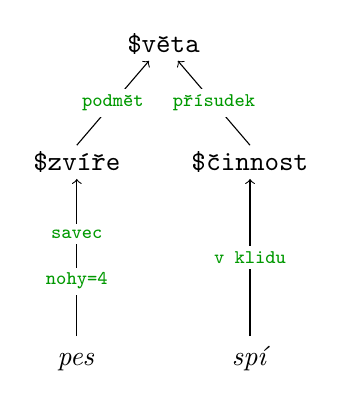
\begin{tikzpicture}[inner sep=2pt]
		\node (pes) at (0, 0) {\strut\emph{pes}};
		\node (spí) at (2.2, 0) {\strut\emph{spí}};
		\node (zvíře) at (0, 2.5) {\texttt{\$zvíře}};
		\node (činnost) at (2.2, 2.5) {\texttt{\$činnost}};
		\node (věta) at (1.1, 4) {\texttt{\$věta}};
		\draw[->] (pes.north) --
		node[pos=0.35, green!60!black,fill=white] {\scriptsize \texttt{nohy=4}}
		node[pos=0.65, green!60!black,fill=white] {\scriptsize \texttt{savec}}
		(zvíře.south);
		\draw[->] (spí.north) -- node[midway,green!60!black, fill=white] {\scriptsize \texttt{v klidu}} (činnost.south);
		\draw[->] (zvíře.north) -- node[midway, green!60!black,fill=white] {\scriptsize \texttt{podmět}} (věta);
		\draw[->] (činnost.north) -- node[midway, green!60!black, fill=white] {\scriptsize \texttt{přísudek}} (věta);
	\end{tikzpicture}
	\hspace{1cm}
	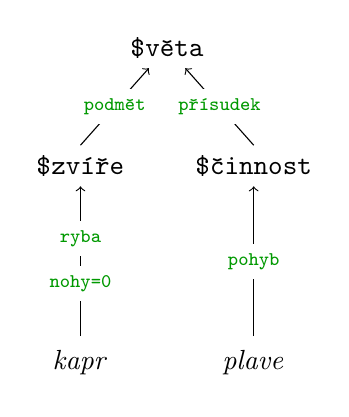
\begin{tikzpicture}
		\node (kapr) at (0, 0) {\strut\emph{kapr}};
		\node (plave) at (2.2, 0) {\strut\emph{plave}};
		\node (zvíře) at (0, 2.5) {\texttt{\$zvíře}};
		\node (činnost) at (2.2, 2.5) {\texttt{\$činnost}};
		\node (věta) at (1.1, 4) {\texttt{\$věta}};
		\draw[->] (kapr.north) --
		node[pos=0.35, green!60!black,fill=white] {\scriptsize \texttt{nohy=0}}
		node[pos=0.65, green!60!black,fill=white] {\scriptsize \texttt{ryba}}
		(zvíře.south);
		\draw[->] (plave.north) -- node[midway,green!60!black, fill=white] {\scriptsize \texttt{pohyb}} (činnost.south);
		\draw[->] (zvíře.north) -- node[midway, green!60!black,fill=white] {\scriptsize \texttt{podmět}} (věta);
		\draw[->] (činnost.north) -- node[midway, green!60!black, fill=white] {\scriptsize \texttt{přísudek}} (věta);
	\end{tikzpicture}
	\hspace{1cm}
	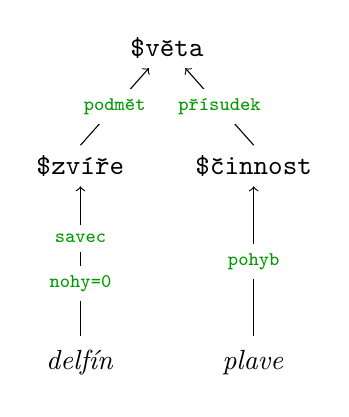
\begin{tikzpicture}
		\node (delfín) at (0, 0) {\strut\emph{delfín}};
		\node (plave) at (2.2, 0) {\strut\emph{plave}};
		\node (zvíře) at (0, 2.5) {\texttt{\$zvíře}};
		\node (činnost) at (2.2, 2.5) {\texttt{\$činnost}};
		\node (věta) at (1.1, 4) {\texttt{\$věta}};
		\draw[->] (delfín.north) --
		node[pos=0.35, green!60!black,fill=white] {\scriptsize \texttt{nohy=0}}
		node[pos=0.65, green!60!black,fill=white] {\scriptsize \texttt{savec}}
		(zvíře.south);
		\draw[->] (plave.north) -- node[midway,green!60!black, fill=white] {\scriptsize \texttt{pohyb}} (činnost.south);
		\draw[->] (zvíře.north) -- node[midway, green!60!black,fill=white] {\scriptsize \texttt{podmět}} (věta);
		\draw[->] (činnost.north) -- node[midway, green!60!black, fill=white] {\scriptsize \texttt{přísudek}} (věta);
	\end{tikzpicture}
	\caption{Derivační stromy s tagy}\label{fig:derivacni_stromy_tagy}
\end{figure}

\todo{doplnit (někam) formální definici syntaxe, případně jako přílohu?}
% Formální definice syntaxe ve formátu ABNF je dána takto:
% \todo{doplnit referenci na ABNF způsob zadávání syntaxe + zkontrolovat, že to odpovídá}
% \todo{doplnit zbytek formální definici syntaxe v ABNF formátu}
% \todo{dát formální definici jako přílohu?}
% \todo{vyměnit za poctivý listing}
% \begin{verbatim}
%     grammar ::= rule+
%     rule ::= ('public' ' ')? ruleName '=' ruleBody ';'
%     ruleName ::= '$' unicodeAlphanumerical+
%     ruleBody ::= ruleAlternative ('|' ruleAlternative)*
%     ruleAlternative ::= element (' ' element)*
%     element ::= token | ruleRef | sequence
%     sequence ::= bracedSequence | optionalSequence
%     bracedSequence ::= '(' bareSequence ')'
%     optionalSequence ::= '[' bareSequence ']'
%     bareSequence ::= ruleAlternative ('|' ruleAlternative)*
% \end{verbatim}

\subsubsection{Vstupní a výstupní body SPGF gramatiky}
\todo{lepší název kapitoly}
Základní rozdíl v parsovací strategii SPGF oproti SRGS spočívá v tom, co je považováno za úspěšný konec parsování.
SRGS implementace
\todo{referovat konkrétně na SC?\@+ ověřit faktickou správnost}
jako úspěšně dokončené parsování považuje takové situace, kde poskytnutý text byl
pokryt daným pravidlem, obojí (pravidlo i text) vyčerpané (využité) beze zbytku od začátku do konce.
Naproti tomu SPGF parser nekontroluje využití celého textu, pouze celého pravidla.
Pokud tedy pravidlo pokryje pouze prvních několik slov a zbytek textu nebude \enquote{pasovat},
SRGS bude tuto situaci brát jako za neúspěch, zatímco SPGF to bude považovat za úspěch.

Dalším rozdílem mezi SRGS a SPGF je ten, že SRGS gramatiky poskytují pouze jeden vstupní bod (pravidlo označené klíčovým slovem \texttt{root}).
Z toho pak plyne, že implementace SRGS mohou pro jeden vstupní text vrátit nejvýše jeden parsovací strom.
\todo{ověřit?}

SPGF oproti tomu umožňuje specifikovat více pravidel jako \enquote{veřejná} klíčovým slovem \texttt{public} a tím tak gramatika bude mít více vstupních bodů.
Parser po načtení SPGF gramatiky vezme všechna pravidla označená jako \texttt{public} a pokusí se pomocí nich zpracovat poskytnutý text.
Výsledky úspěšných parsování jsou pak vrácené jako výstupy v podobě derivačních stromů, se kterými je možné dále pracovat.

Pro příklad uvažujme vstupní text: \enquote{\emph{hnědý pes utíká pryč}} a gramatiku na Listing~\ref{lst:simple_grammar_1}.
\todo{zlepšit barvy}
\begin{lstlisting}[
	% there are many more options of styling, see the official documentation, these are just the defaults I like
	frame=single, % make single-line frame around the verbatim
	framesep=2mm, % put some more spacing between the frame and text
	aboveskip=5mm, % put some more space above the box
	basicstyle={\linespread{1.0}\small\ttfamily}, % use typewriter (monospace) font
	caption={Ukázková SPGF gramatika}, % set the caption text
	captionpos=b, % put the caption at the bottom (b) or top (t) or both (bt)
	label={lst:simple_grammar_1}, % label to be referenced via \ref{}
	numbers=left, % line numbers on the left
	numberstyle={\scriptsize\ttfamily\color{black!60}}, % the style for line numbers
	escapeinside={<@}{@>} % between those sequences are command evaluated
]
<@\textcolor[HTML]{8839EF}{\texttt{public}}@><@\textcolor[HTML]{000000}{\texttt{\ }}@><@\textcolor[HTML]{255CFF}{\texttt{\$sentence\ =}}@><@\textcolor[HTML]{000000}{\texttt{\ }}@><@\textcolor[HTML]{724BFF}{\texttt{\$color}}@><@\textcolor[HTML]{000000}{\texttt{\ }}@><@\textcolor[HTML]{724BFF}{\texttt{\$object}}@><@\textcolor[HTML]{000000}{\texttt{\ }}@><@\textcolor[HTML]{724BFF}{\texttt{\$action}}@><@\textcolor[HTML]{1041FF}{\textbf{\texttt{;}}}@>
<@\textcolor[HTML]{255CFF}{\texttt{\$color\ =}}@><@\textcolor[HTML]{000000}{\texttt{\ modrý\ }}@><@\textcolor[HTML]{1041FF}{\textbf{\texttt{|}}}@><@\textcolor[HTML]{000000}{\texttt{\ zelený\ }}@><@\textcolor[HTML]{1041FF}{\textbf{\texttt{|}}}@><@\textcolor[HTML]{000000}{\texttt{\ hnědý}}@><@\textcolor[HTML]{1041FF}{\textbf{\texttt{;}}}@>
<@\textcolor[HTML]{255CFF}{\texttt{\$object\ =}}@><@\textcolor[HTML]{000000}{\texttt{\ pes\ }}@><@\textcolor[HTML]{1041FF}{\textbf{\texttt{|}}}@><@\textcolor[HTML]{000000}{\texttt{\ míč\ }}@><@\textcolor[HTML]{1041FF}{\textbf{\texttt{|}}}@><@\textcolor[HTML]{000000}{\texttt{\ autobus}}@><@\textcolor[HTML]{1041FF}{\textbf{\texttt{;}}}@>
<@\textcolor[HTML]{255CFF}{\texttt{\$action\ =}}@><@\textcolor[HTML]{000000}{\texttt{\ utíká\ }}@><@\textcolor[HTML]{1041FF}{\textbf{\texttt{|}}}@><@\textcolor[HTML]{000000}{\texttt{\ jede\ }}@><@\textcolor[HTML]{1041FF}{\textbf{\texttt{|}}}@><@\textcolor[HTML]{000000}{\texttt{\ [se]\ kutálí}}@><@\textcolor[HTML]{1041FF}{\textbf{\texttt{;}}}@>

\end{lstlisting}


Tuto gramatiku z Listing~\ref{lst:simple_grammar_1} lze zakreslit jako konečný automat
na Obrázku~\ref{fig:scheme_grammar_final_automata}.
\begin{figure}[H]
	\centering
	\begin{tikzpicture}[inner sep=0pt, rounded corners=2mm]
		\node[draw, minimum width=17mm] (modrý) at (0, 1)  {\texttt{\strut modrý}};
		\node[draw, minimum width=17mm] (zelený) at (0, 0) {\texttt{\strut zelený}};
		\node[draw, minimum width=17mm] (hnědý) at (0, -1) {\texttt{\strut hnědý}};
		\node[fill, circle, minimum width=5pt] (start) at ($(zelený.west) + (-1, 0)$) {};

		\node[draw, minimum width=20mm, anchor=west] (pes) at ($(modrý.east) + (1.5, 0)$)  {\texttt{\strut pes}};
		\node[draw, minimum width=20mm, anchor=west] (míč) at ($(zelený.east) + (1.5, 0)$) {\texttt{\strut míč}};
		\node[draw, minimum width=20mm, anchor=west] (autobus) at ($(hnědý.east) + (1.5, 0)$) {\texttt{\strut autobus}};

		\node[draw, minimum width=20mm, anchor=west] (utíká) at ($(pes.east) + (3.5, 0)$)  {\texttt{\strut utíká}};
		\node[draw, minimum width=20mm, anchor=west] (jede) at ($(míč.east) + (3.5, 0)$) {\texttt{\strut jede}};
		\node[draw, minimum width=20mm, anchor=west] (kutálí) at ($(autobus.east) + (3.5, 0)$) {\texttt{\strut kutálí}};

		\node[draw, minimum width=10mm, anchor=east] (se) at ($(kutálí.west) + (-1, 0)$) {\texttt{\strut se}};

		\node[fill, circle, minimum width=5pt] (end) at ($(jede.east) + (1.1, 0)$) {};

		\draw[-Stealth] (start.center) -- ($(zelený.west) + (-0.5, 0)$) -- ($(modrý.west) + (-0.5, 0)$) -- (modrý.west);
		\draw[-Stealth] (start.center) -- ($(zelený.west) + (-0.5, 0)$) -- ($(hnědý.west) + (-0.5, 0)$) -- (hnědý.west);
		\draw[-Stealth] (start.center) -- (zelený.west);

		\draw[-Stealth] (modrý.east)
		-- ($(modrý.east) + (0.5, 0)$)
		-- ($(zelený.east) + (0.5, 0)$)
		-- ($(míč.west) + (-0.5, 0)$)
		-- ($(pes.west) + (-0.5, 0)$)
		-- (pes.west);
		\draw[-Stealth] (hnědý.east)
		-- ($(hnědý.east) + (0.5, 0)$)
		-- ($(zelený.east) + (0.5, 0)$)
		-- ($(míč.west) + (-0.5, 0)$)
		-- ($(autobus.west) + (-0.5, 0)$)
		-- (autobus.west);
		\draw[-Stealth] (zelený.east) -- (míč.west);

		\draw[-Stealth] (pes.east)
		-- ++(0.5, 0)
		-- ++(0, -1)
		-- ($(jede.west) + (-0.5, 0)$)
		-- ++(0, 1)
		-- (utíká.west);
		\draw[-Stealth] (autobus.east)
		-- ++(0.5, 0)
		-- ++(0, 1)
		-- ($(jede.west) + (-0.5, 0)$)
		-- ++(0, -1)
		-- (kutálí.west);
		\draw[-Stealth] (míč.east) -- (jede.west);
		\draw[-Stealth] ($(se.west) + (-1, 1)$)
		-- ($(se.west) + (-0.5, 1)$)
		-- ($(se.west) + (-0.5, 0)$)
		-- (se.west);
		\draw[-Stealth] (se.east) -- (kutálí.west);

		\draw[-Stealth] (jede.east) -- (end);
		\draw[-Stealth] (utíká.east) -- ++(0.5, 0) -- ++(0, -1) -- (end);
		\draw[-Stealth] (kutálí.east) -- ++(0.5, 0) -- ++(0, 1) -- (end);
	\end{tikzpicture}
	\caption{Schéma gramatiky jako konečného automatu}\label{fig:scheme_grammar_final_automata}
\end{figure}

Při zpracování textu by mohl vzniknout následující derivační strom, který je na Obrázku~\ref{fig:parsing_tree_example}:
\begin{figure}[H]
	\centering
	\begin{tikzpicture}[anchor=west,inner sep=2pt]
		\def\spacing{40pt}
		\node (w1) at (0,0) {\strut\emph{hnědý}};
		\node (w2) at ($(w1.east) + (\spacing, 0)$) {\strut\emph{pes}};
		\node (w3) at ($(w2.east) + (\spacing, 0)$) {\strut\emph{utíká}};
		\node (w4) at ($(w3.east) + (\spacing, 0)$) {\strut\emph{pryč}};
		\node[anchor=center] (n1) at ($(w1.center) + (0, \spacing)$) {\texttt{\strut\$color}};
		\node[anchor=center] (n2) at ($(w2.center) + (0, \spacing)$) {\texttt{\strut\$object}};
		\node[anchor=center] (n3) at ($(w3.center) + (0, \spacing)$) {\texttt{\strut\$action}};
		\node[anchor=center] (n4) at ($0.5*(n1.west) + 0.5*(n3.east) + (0, \spacing)$) {\texttt{\strut\$sentence}};
		\draw[->] (w1) to (n1);
		\draw[->] (w2) to (n2);
		\draw[->] (w3) to (n3);
		\draw[->] (n1) to (n4);
		\draw[->] (n2) to (n4);
		\draw[->] (n3) to (n4);
	\end{tikzpicture}
	\caption{Ukázkový derivační strom}\label{fig:parsing_tree_example}
\end{figure}

Jak je vidět, poslední slovo \enquote{\emph{pryč}} není součástí derivačního stromu,
protože parsovací pravidlo \texttt{\$sentence} jej nedokáže pokrýt.
V případě SRGS by tento derivační strom byl považovaný za neúspěch, zatímco SPGF vrátí zobrazený parsovací strom
jako úspěšný výsledek.

\subsubsection{Parsovací strategie SPGF}
